\documentclass[tikz,border=10pt]{standalone}
\usepackage{amsmath,amssymb}
\usepackage{tikz}
\usetikzlibrary{arrows,automata,backgrounds,calendar,chains,decorations,decorations.pathreplacing,decorations.text,fit,matrix,mindmap,patterns,petri,plotmarks,positioning,shadows,shapes,shapes.callouts,shapes.geometric,shapes.misc,spy,trees,calc,intersections,tikzmark,arrows.meta}
\usepackage{xcolor}
\usepackage{pgfplots}
\pgfplotsset{compat=1.16}

% Common math macros from the book
\def\x{\mathbf{x}}
\def\y{\mathbf{y}}
\def\z{\mathbf{z}}
\def\A{\mathbf{A}}
\def\b{\mathbf{b}}
\def\c{\mathbf{c}}
\def\w{\mathbf{w}}
\def\v{\mathbf{v}}
\def\u{\mathbf{u}}
\def\e{\mathbf{e}}
\def\zero{\mathbf{0}}
\def\R{\mathbb{R}}
\def\N{\mathbb{N}}
\def\Z{\mathbb{Z}}
\def\Q{\mathbb{Q}}
\def\st{\text{s.t.}}
\def\vect#1{\mathbf{#1}}
\def\xLP{x^{\mathrm{LP}}}
\def\zLP{z^{\mathrm{LP}}}
\def\xIP{x^{\mathrm{IP}}}

% Common node styles from the book
\tikzset{
    main/.style={circle, draw, fill=gray!20, minimum size=1cm, font=\normalsize},
    dot/.style={circle,fill=blue,minimum size=3pt,inner sep=0pt, outer sep=-1pt},
    vertex/.style={circle,fill=black!25,minimum size=20pt,inner sep=0pt},
    edge/.style={draw,-,thick},
    directed edge/.style={draw,->,>=latex,thick},
}

% Additional macros for 3D/coordinate systems
\newcommand{\xhat}{\hat{\x}}
\newcommand{\yhat}{\hat{\y}}
\newcommand{\zhat}{\hat{\z}}
\newcommand{\ihat}{\hat{\imath}}
\newcommand{\jhat}{\hat{\jmath}}
\newcommand{\khat}{\hat{k}}

\begin{document}
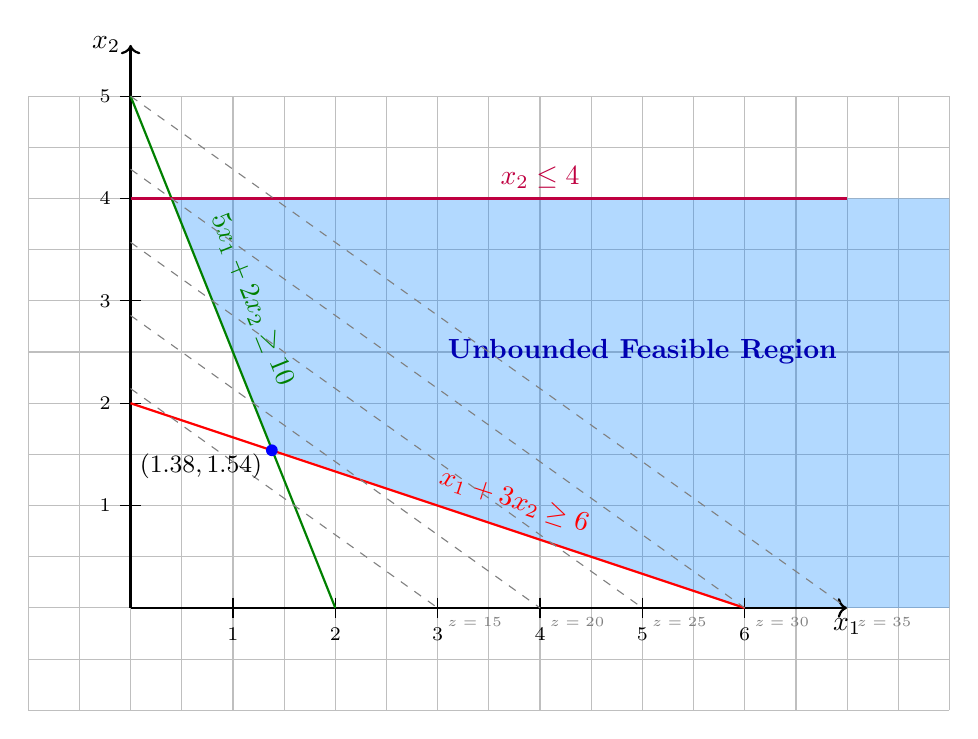
\begin{tikzpicture}[scale = 1.3]
    \draw[gray!50, thin, step=0.5] (-1,-1) grid (8,5);

    % Highlight the feasible region
    \fill[blue!50!cyan,opacity=0.3] 
        (0.4,4) -- (1.39,1.55)  -- (6,0) -- (8,0) -- (8,4) -- cycle;

    % Define axes
    \draw[thick,->] (0,0) -- (7,0) node[anchor=north] {$x_1$};
    \draw[thick,->] (0,0) -- (0,5.5) node[anchor=east] {$x_2$};

    % Add tick marks on the x_1-axis
    \foreach \x in {1,2,3,4,5,6} {
        \draw (\x,0.1) -- (\x,-0.1) node[anchor=north] {\scriptsize $\x$};
    }

    % Add tick marks on the x_2-axis
    \foreach \y in {1,2,3,4,5} {
        \draw (0.1,\y) -- (-0.1,\y) node[anchor=east] {\scriptsize $\y$};
    }

    % Define the constraints
    % Line 1: X + 3Y = 6
    \draw[red,thick] (0,2) -- (6,0);
    \node[red, rotate=-18, anchor=north west] at (3,1.5) {$x_1 + 3x_2 \geq 6$};

    % Line 2: 5X + 2Y = 10
    \draw[green!50!black,thick] (0,5) -- (2,0);
    \node[green!50!black, rotate=-68, anchor=north west] at (1,4) {$5x_1 + 2x_2 \geq 10$};

    % Line 3: Y = 4
    \draw[purple,thick] (0,4) -- (7,4);
    \node[purple, rotate=0, anchor=south] at (4,4) {$x_2 \leq 4$};

    % Label feasible region
    \node[blue!70!black, font=\bfseries] at (5,2.5) {Unbounded Feasible Region};

    % Mark intersection points
%    \fill[black] (0,4) circle (2pt) node[anchor=east] {\scriptsize $(0,4)$};
%    \fill[black] (6,0) circle (2pt) node[anchor=north] {\scriptsize $(6,0)$};

% Objective function contours
\foreach \c in {15,20,25,30,35} {
    \draw[dashed,gray] (0,\c/7) -- (\c/5,0) node[below right] {\tiny$z = \c$};
    }
%    \draw[dashed,gray] (0,3) -- (1.5,0) node[below right] {\tiny$c = 7.5$};
%    \draw[dashed,gray] (0,2) -- (1,0) node[below right] {\tiny$c = 5$};
%    \draw[dashed,gray] (0,1) -- (0.5,0) node[below right] {\tiny$c = 2.5$};
%    \draw[dashed,gray] (0,0) -- (0,0) node[below right] {\tiny$c = 0$};

    % Contour labels
    %\node[gray] at (0.5,3.5) {\tiny$3x_1 + 2x_2 = c$};
\node[blue,circle,fill,inner sep=1.5pt,label={[black,anchor=north east]\small$(1.38,1.54)$}] at (1.38,1.54) {};

\end{tikzpicture}
\end{document}
